\newpage
\section{Calculations}

\begin{figure}[!h]
  \centering
  \begin{subfigure}{0.6\textwidth}
    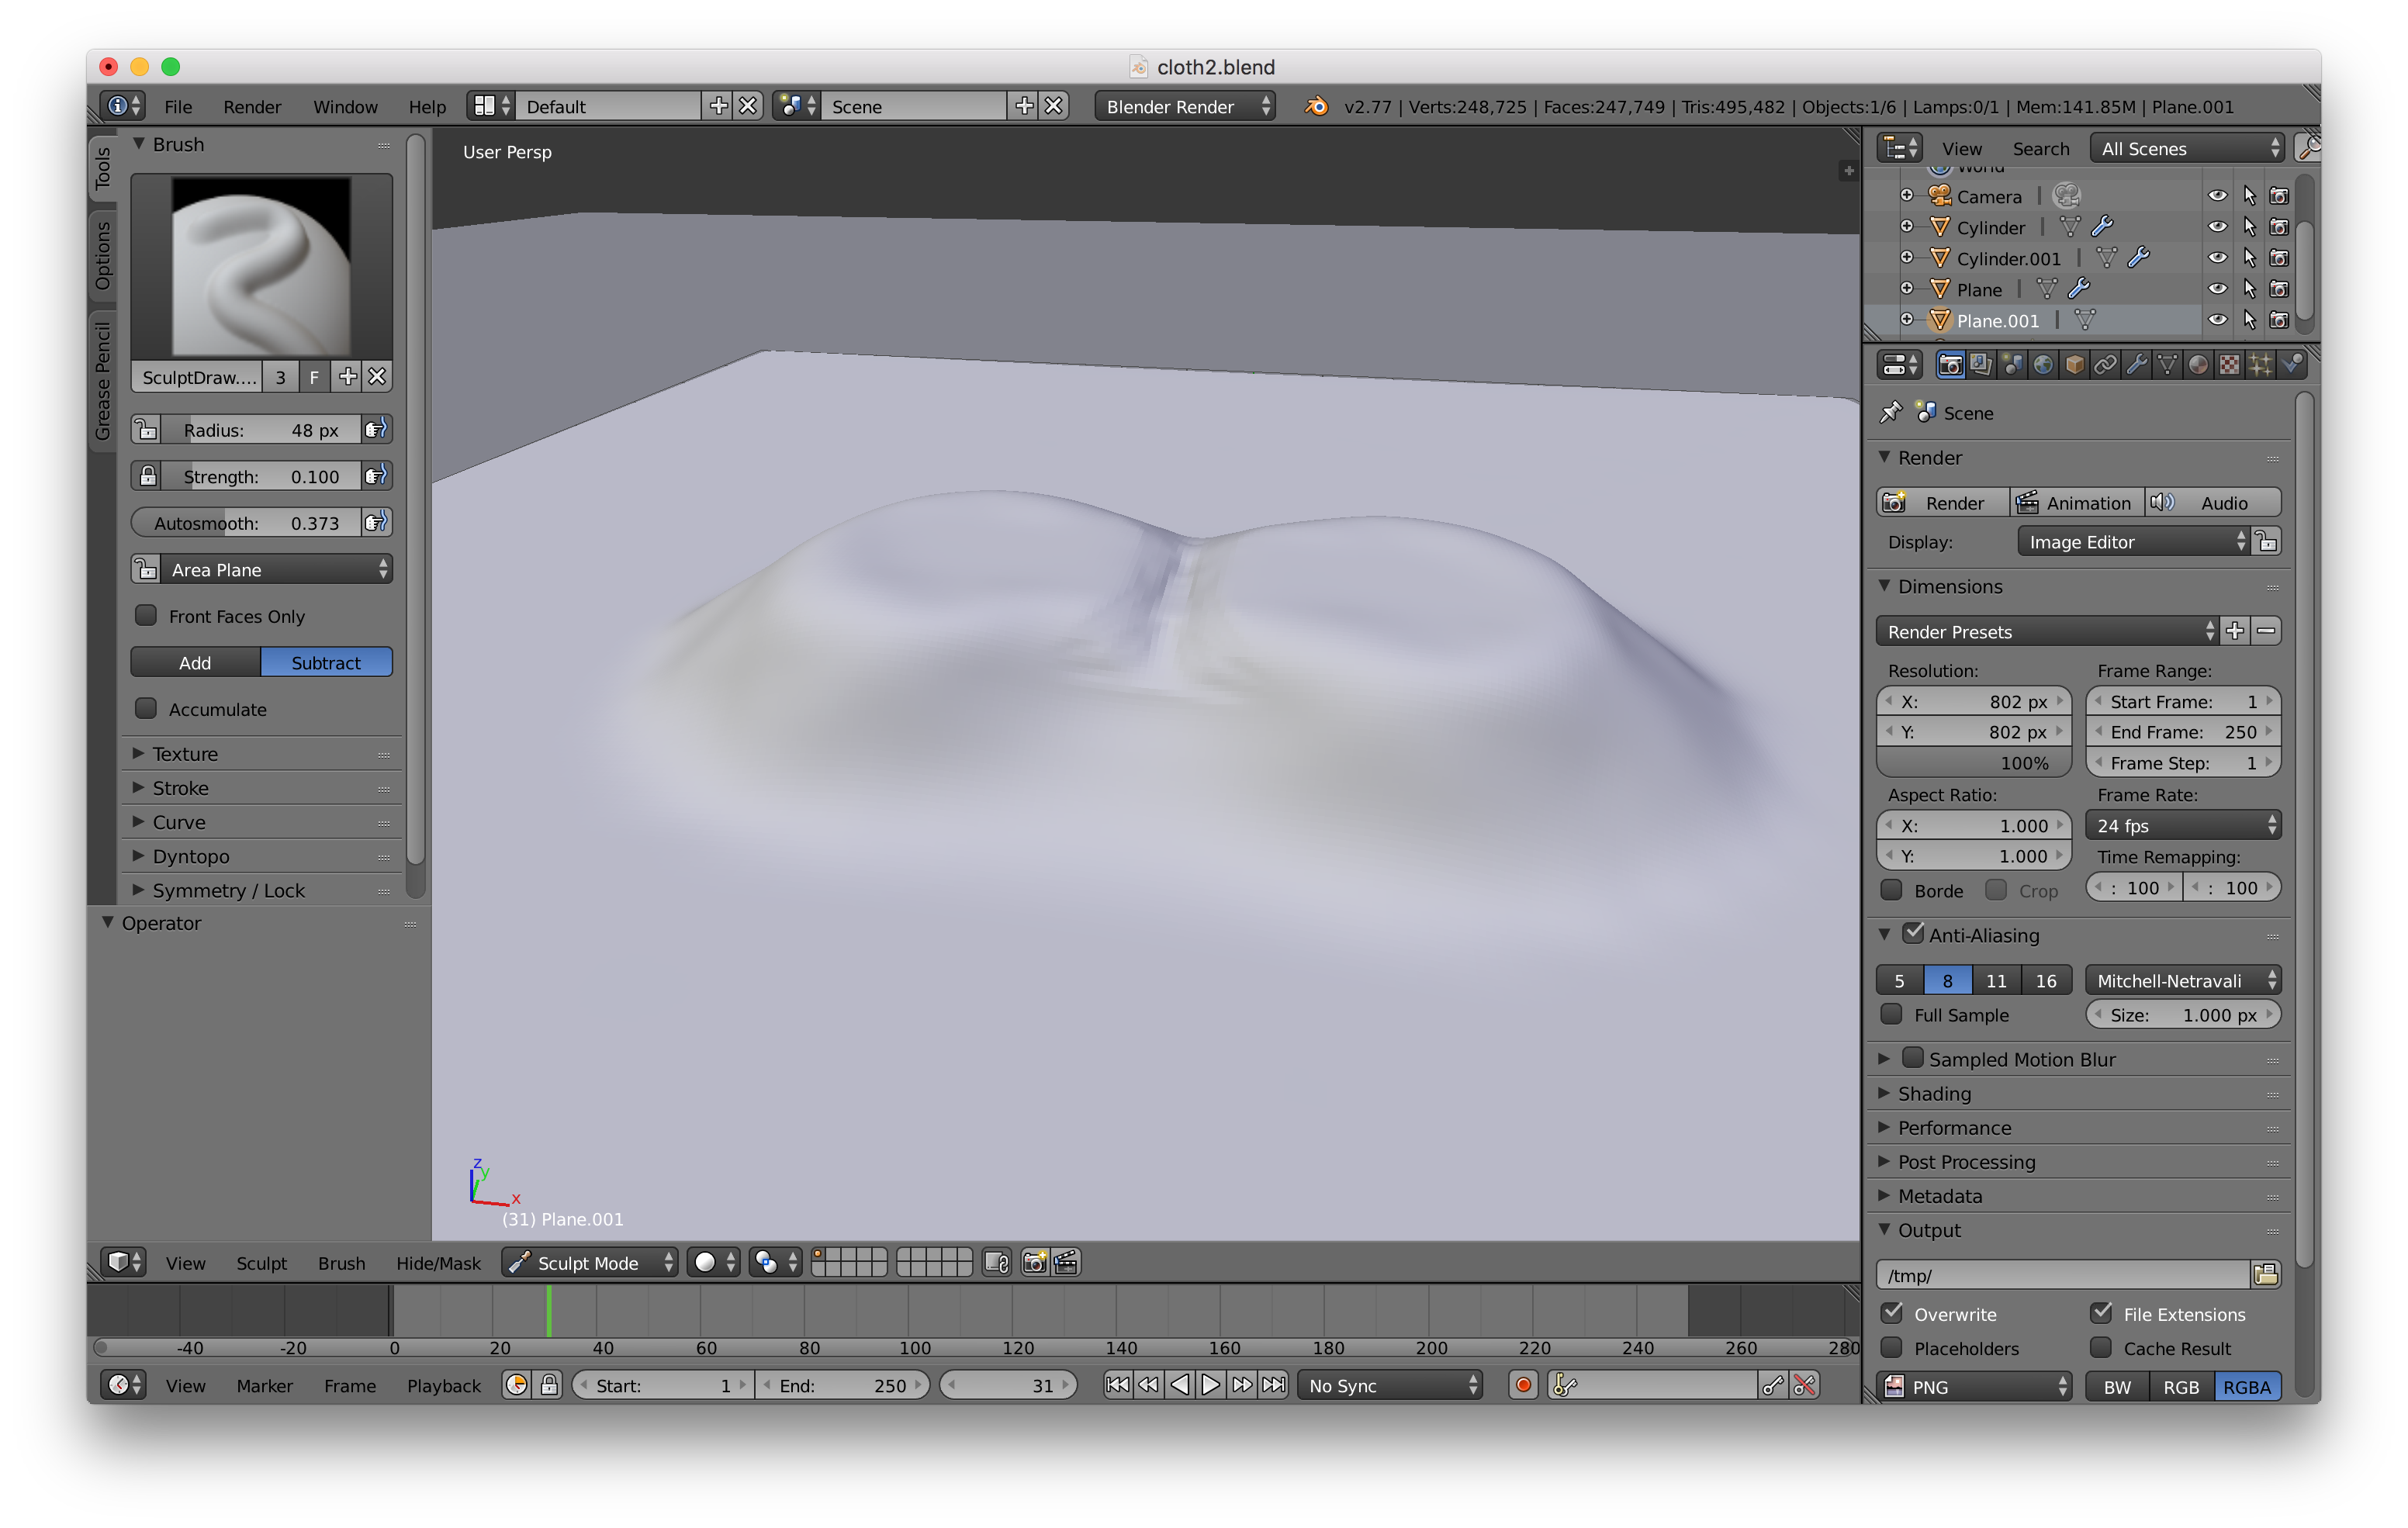
\includegraphics[width=\textwidth]{./images/blender.png}
  \end{subfigure}
  ~
  \begin{subfigure}{0.35\textwidth}
    
\includegraphics[width=\textwidth]{./images/map.png}
  \end{subfigure}
  \caption{\textbf{(a)} Cloth simulation in Blender 2.7. An elastic material is dropped on 2 cylinders with a radius of \SI{50}{nm}. \textbf{(b)} A generated heightmap after rendering. Black corresponds to 0, white to maximum height.}
\end{figure}
